\documentclass{article}
\usepackage{geometry}
\usepackage{float}
\usepackage[T1]{fontenc}
\usepackage[polish]{babel}
\usepackage[utf8]{inputenc}
\usepackage{graphicx}
\graphicspath{ {./images/} }

\geometry{
 a4paper,
 total={170mm,257mm},
 left=20mm,
 top=20mm,
}

\title{Analiza i przetwarzanie dźwięku - Projekt 2}
\date{04/05/2020}
\author{Mateusz Śliwakowski}

\begin{document}
  \pagenumbering{gobble}
  \maketitle
  \pagenumbering{arabic}
  
\section{Treść zadania}

\section{Opis aplikacji}

Aplikację zdecydowałem się wykonać w języku \textit{C\#} w środowisku \textit{WinForms}. Całość zacząłem od zaprojektowania wyglądu interfejsu użytkownika.

\section{Implementacja}

\section{Wyniki działania programu}

\section{Wnioski}

\begin{figure}[b]
\centering
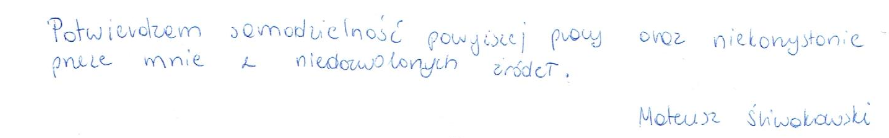
\includegraphics[width=5in]{bottom.png}
\end{figure}

\end{document}

